\documentclass[12pt]{article}

\usepackage{fontawesome}
\usepackage{hyperref}
\usepackage{xurl}
\usepackage{graphicx}


\hypersetup{
    colorlinks=false,
    pdfborder={0 0 0},
}


\title{Data Laws and Regulations}
\author{
        Adrianna Holden-Gouveia \\
        Website: \url{https://aholdengouveia.name}\\ 
        \date{\vspace{-5ex}}
        %Email: \href{mailto:admin@aholdengouveia.name}{admin@aholdengouveia.name} \\
        \faLinkedin{: aholdengouveia} \\
        \faGithub {: aholdengouveia} \\
        %\faTwitter {: aholdengouveia} \\
        }

%S\date{\today}


\begin{document}    

\maketitle

%\begin{abstract}
%This is a template for Linux Administration Lab work
%\end{abstract}
%\tableofcontents

\section*{Objectives:}
\begin{itemize}
    \item Students will gain a holistic understanding of data privacy, regulations, and their global implications through practical and hands on activities.
\end{itemize}
\section*{Complete the following problems}

References, a video, a PowerPoint and some notes are available at my website
\url {https://www.aholdengouveia.name/IntroData/datalawsandregs.html}


\subsection*{Privacy Policy Analysis}

You are tasked with analyzing the privacy policies of a popular social media platform.  Pick one of the following options: 
        \begin{itemize}
            \item Facebook: \url{https://www.facebook.com/}
            \item TikTok: \url{https://www.tiktok.com/}
            \item Instagram: \url{https://www.instagram.com/}
            \item WhatsApp: \url{https://www.whatsapp.com/}
            \item SnapChat: \url{https://www.snapchat.com/}
            \item Pinterest: \url{https://www.pinterest.com/}
            \item LinkedIn: \url{https://www.linkedin.com/}
    \end{itemize}
        
        

Using the privacy policy from their website, read it through carefully and answer the following questions.  Each answer should include a screenshot of the relevant section(s) on the policy

Each screenshot should have your name, term, and year.  One of the easiest ways to do that is make a text document with your name and term/year on your computer and saving it to use all term. Any screenshots that don't include this information won't be counted.

\begin{figure}[h!]
    \centerline{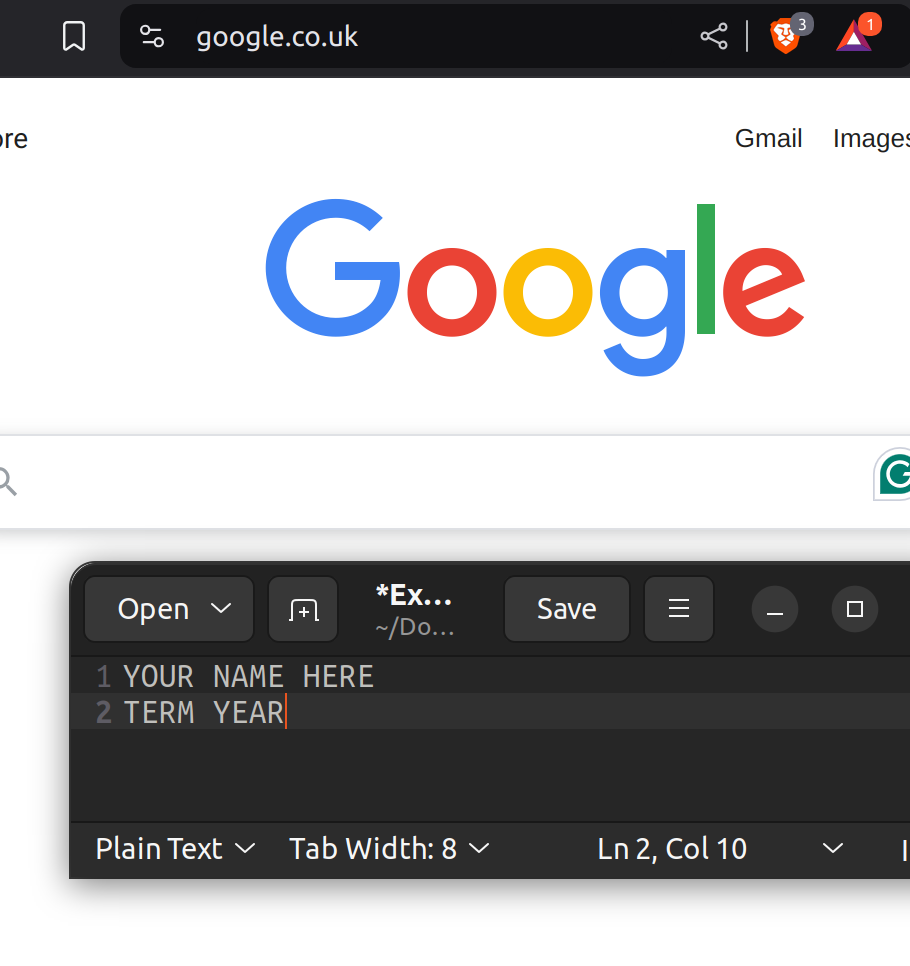
\includegraphics[scale=.2]{ExampleScreenshot.png}}
    \caption{This is an image of what each of your screenshots should look like}

    \end{figure} 
            \begin{enumerate}
                \item What is the link to their privacy policy? If there are more than 1, include all links.
                \item What types of data are collected from users?  Make a list.
                \item How is the collected data used by the platform?  Make a list or table.
                \item Is user data shared with third parties? If so, for what purposes?
                \item What rights do users have regarding their personal data?
                \item If there is an issue, what are the options for litigation? What steps are detailed in the policy that cover legal recourse for bad practices?
                \item Would the options for Litigation change if you were an EU citizen? What about citizen of another country outside the USA or EU?
                \item What age does the platform consider "child"? Does that change how the data is handled?
                \item What measures does the platform take to ensure the security of user data?
                \item What are the options for users to control their privacy settings?
                \item Does the platform use cookies or tracking technologies?
                \item What are the data retention policies of the platform?
                \item How does the platform handle user consent and opt-in/opt-out mechanisms?
        \end{enumerate}


\section*{Deliverables}

\begin{enumerate}
    \item Which social media platform you picked, and why.
    \item Link to the platform, link to the privacy policy(s)
    \item Answers to the questions listed above with their screenshots.

\end{enumerate}

\end{document}